\documentclass[amsmath,amssymb,showpacs,prf,superscriptaddress,notitlepage,longbibliography]{revtex4-1}
%\documentclass[amsmath,amssymb,showpacs,prl,superscriptaddress,notitlepage]{revtex4-1}
\bibstyle{apsrev}

\usepackage{graphics,graphicx,dcolumn,bm,fleqn,epic,eepic,float}
\usepackage{amssymb,amsmath,multirow,rotate,rotating,color}
\usepackage[utf8]{inputenc}

\usepackage[english]{babel}
\usepackage{caption}
\usepackage{subcaption}
\usepackage{tikz}
\usepackage{hyperref}
\hypersetup{
    colorlinks=true,
    linkcolor=blue,
    filecolor=magenta,      
    urlcolor=cyan,
}
%\usepackage[usenames,dvipsnames,svgnames,table]{xcolor}
\tikzset{fontscale/.style = {font=\relsize{#1}}}
\usetikzlibrary{calc}
\usepackage{color}
\usepackage{xcolor}
\usepackage{physics}
%\usepackage[colorlinks=true,linkcolor=blue]{hyperref}%
\hyphenation{title}

\begin{document}

\definecolor{pyblue}{HTML}{1F77B4}
\definecolor{pyorange}{HTML}{FF7F0C}
\definecolor{pygreen}{HTML}{2CA02C}
\definecolor{pyred}{HTML}{D62728}
\definecolor{jlblue}{rgb}{0.0,0.6056031611752245,0.9786801175696073}
\definecolor{jlorange}{rgb}{0.8888735002725198,0.43564919034818994,0.2781229361419438}
\newcommand*\Diff[1]{\mathop{}\!\mathrm{d^#1}}

\title{Controlling the dewetting morphologies of thin liquid films by switchable substrates: Supplemental Material}

\author{S. Zitz}
\email{zitz@ruc.dk}
 %Changed order: Work done while Stefan worked in Nuremberg
 \affiliation{Helmholtz Institute Erlangen-N\"urnberg for Renewable Energy,\\
  Forschungszentrum J\"ulich,
  F\"urther Strasse 248, 90429 N\"urnberg, Germany}%
  \affiliation{Department of Chemical and Biological Engineering, Friedrich-Alexander-Universit\"at Erlangen-N\"urnberg, F\"{u}rther Stra{\ss}e 248, 90429 N\"{u}rnberg, Germany}
  \affiliation{IMFUFA, Department of Science and Environment,\\ 
Roskilde University, Postbox 260, DK-4000 Roskilde, Denmark}%
\author{A. Scagliarini}%
\email{andrea.scagliarini@cnr.it}
 \affiliation{Institute for Applied Mathematics "M. Picone" (IAC), 
Consiglio Nazionale delle Ricerche (CNR),\\
Via dei Taurini 19, 00185 Rome, Italy}%
\affiliation{INFN, sezione Roma ``Tor Vergata'', via della Ricerca Scientifica 1, 00133 Rome, Italy}
\author{J. Harting}
\email{j.harting@fz-juelich.de}
 \affiliation{Helmholtz Institute Erlangen-N\"urnberg for Renewable Energy,\\
  Forschungszentrum J\"ulich,
  F\"urther Strasse 248, 90429 N\"urnberg, Germany}%
 \affiliation{Department of Chemical and Biological Engineering and Department of Physics, Friedrich-Alexander-Universit\"at Erlangen-N\"urnberg, F\"{u}rther Stra{\ss}e 248, 90429 N\"{u}rnberg, Germany}
\date{\today}

\maketitle

\section{Disjoining pressure}

\noindent A {\it thin film} is a layer of liquid confined between two interfaces. When the two interfaces are brought close enough to each other (i.e. the layer is {\it thin}), they interact.
The disjoining pressure stems from this interaction. Thermodynamically, it represents minus the derivative of the free energy difference, per unit surface, between 
the film and the bulk of the same liquid, or, equivalently, the pressure difference inside and outside the film \cite{Deryaguin1940,DeryaguinChuraev1978}.
In the case of wetting, there can be three types of interfaces: liquid/air, liquid/solid (the substrate) and, if the substrate is only partially wetted, solid/air, thus giving rise to three-phase contact lines. 
The usually called "surface tension" is the energy cost of forming a liquid/air interface of unit area. 
The Young's condition \cite{youngIIIEssayCohesion1805,degennesWettingStaticsDynamics1985} connects the surface tension with the analogous energies per unit area associated with the solid/liquid ($\gamma_{\text{sl}}$) and solid/gas ($\gamma_{\text{sg}}$) interface as
\begin{equation}
\cos \theta = \frac{\gamma_{\text{sg}}-\gamma_{\text{sl}}}{\gamma},
\end{equation}
where $\theta$ is the contact angle.
The expression adopted for $\Pi$, namely
\begin{equation}
\Pi(h,\theta) = \frac{2\gamma}{h_{\ast}}(1-\cos(\theta(\mathbf{x},t)))
  f\left(\frac{h}{h_{\ast}}\right),
\end{equation}
where $f(\xi)=\xi^{-3} - \xi^{-2}$ and $h_{\ast}$ is the height at which the disjoining pressure vanishes setting the precursor layer thickness, pertains to a general family of expressions of the form 
\begin{equation}\label{eq:SMDP}
\Pi(h) = \gamma(1-\cos \theta)\frac{(n-1)(m-1)}{h_{\ast}(n-m)}\left[\left(\frac{h_{\ast}}{h}\right)^n - 
\left(\frac{h_{\ast}}{h}\right)^m\right].
\end{equation}
Equations like (\ref{eq:SMDP}) are frequently found in the literature, with various combination of exponents $(n,m)$ ($n>m$), depending on the type of interactions among fluid molecules and between fluid and substrate~\cite{schwartzSimulationDropletMotion1998,mitlinDewettingSolidSurface1993,teletzkeHowLiquidsSpread1987}. 
A common choice, for instance, is the pair $(9,3)$, which can be derived from molecular interactions of Lennard-Jones type. 
Here, the use of the $(3,2)$ pair is motivated mainly by the computational advantage of keeping the characteristic dewetting time shorter. 
We have run also a single case ($\lambda=256 h_0$ and $\Gamma=1.5$) with $(9,3)$ and observed that the dynamics remains essentially the same, but for a shift in the time scale (see also~\cite{zitzLatticeBoltzmannSimulations2021}).

\section{Parameter values and comparison with experiments}\label{sec:SMparam}

\noindent To give a flavour of how to compare with actual experimental systems, let us notice first that the expression of $t_0$ depends on the disjoining pressure (through its dependence $q_0 = \sqrt{\frac{1}{2\gamma} \Pi^{\prime}(h_0)}$) and contains, therefore, energetic details, namely the Hamaker constant $A_H$. 
Consider, for instance, the problem studied in \cite{beckerComplexDewettingScenarios2003}: the dewetting of a polystyrene film of thickness $h_0 \approx 4 \, \text{nm}$ deposited on a silicon dioxide substrate, where $A_H  = 2.2 \times 10^{-20} \, \text{J}$ and $\gamma = 0.03 \, \text{N}/\text{m}$. 
Neglecting the short range part of the interface potential (such that $\Pi(h)= - \frac{A_H}{6\pi h^3}$)~\cite{meckeThermalFluctuationsThin2005,beckerComplexDewettingScenarios2003}, one gets $q_0^2 \approx \frac{A_H}{4\pi \gamma h_0^4} \approx 2.5 \times 10^{-4} \, \text{nm}^{-2}$.
The characteristic time of the growth of the instability for these experiments then reads $t_0 = \frac{3\mu}{\gamma h_0^3 q_0^4} \approx 300 \, \text{s}$ (the dynamic viscosity of polystyrene is $\mu = 1.2 \times 10^4 \, \text{Pa} \cdot \text{s}$)~\cite{fetzerThermalNoiseInfluences2007}. 
It can be seen that indeed film rupture occurs within time scales of the order of $t_0$~\cite{beckerComplexDewettingScenarios2003}, as in our simulation for the largest pattern wavelength, $\lambda = L$ (see also our previous work with homogeneous substrates~\cite{zitzLatticeBoltzmannSimulations2021}).\\
All our simulations are run on a bi-periodic square domain of size $L \times L$ with $L/h_0 = 512 $. 
The numerical values in lattice Boltzmann units of the mean film thickness, dynamics viscosity and surface tension are, respectively, $h_0=1$, $\mu=1/6$ and $\gamma=0.01$.
To regularize the contact line divergence~\cite{huhHydrodynamicModelSteady1971} we use a precursor layer thickness $h_{\ast}/h_0=0.07$ and a slip length $\delta/h_0 = 1$, a value which lies within the weak/intermediate slip regime~\cite{peschkaSignaturesSlipDewetting2019,fetzerQuantifyingHydrodynamicSlip2007, munchLubricationModelsSmall2005a} (we have tried also a value four times smaller, without observing any major qualitative change in the results).
The liquid film is initialized with a height field slightly perturbed around the mean value $h_0$, i.e. $h(\mathbf{x},0) = h_0 \left[1 + 0.1 \left(\sin\left(\frac{2\pi x}{L}\right)\sin\left(\frac{2\pi y}{L}\right)\right)\right]$.
Various wavelengths in the range $\lambda/h_0 \in [64, 512]$, and velocities, $v_{\theta}/v_0 \in [0, 200]$, are considered for the wettability pattern (see main text). 
A few comments on these ranges are noteworthy at this point. The wavelengths are obviously limited from above by the size of the computational domain. 
On the other extreme, too short wavelengths are prevented by the energetic cost of accommodating droplets on too small patches, since the local contact angle (that increases with decreasing $\lambda$, see also Sec.~\ref{sec:SMdroplet}) would possibly exceed the largest substrate contact angle, such that the patterning itself would lose meaning. 
It has been, in fact, proven, both theoretically and experimentally, that for the confinement to be effective, the pattern characteristic size should not be much smaller than the spinodal length scale on the less wettable substrate~\cite{karguptaMorphologicalSelforganizationDewetting2002,karguptaInstabilityPatternFormation2000,nisatoExcitationSurfaceDeformation1999,karimPhaseSeparationUltrathin1998}.
We keep, therefore, $\lambda \stackrel{>}{\sim} \lambda_s \approx 70 h_0$.
The pattern speeds, on the other hand, are limited by the intrinsic LB bound of the lattice speed of sound~\cite{succiLatticeBoltzmannEquation2001}.\\
The Reynolds number, $Re$, is of the order of $Re \sim 10^{-2}$ on the static substrate and never exceeds the value $\approx 0.2$ in the time dependent case.

\section{Minkowski's structure metric \texorpdfstring{$q_2$}{second metric} in an extended parameter space}\label{sec:SMMinko}

\begin{figure}
    \centering
    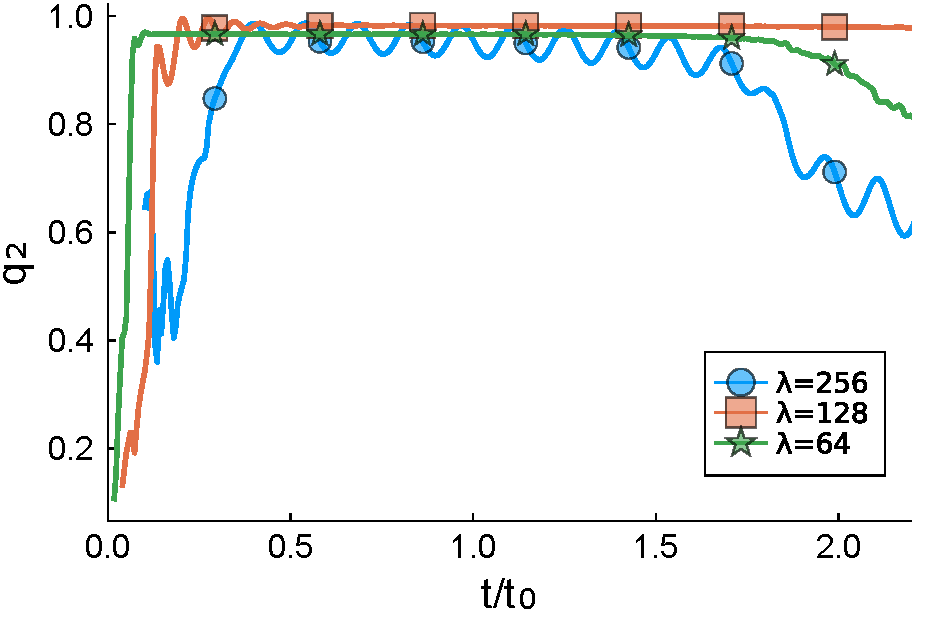
\includegraphics[width=0.4\textwidth]{SupMatFig_1.pdf}
    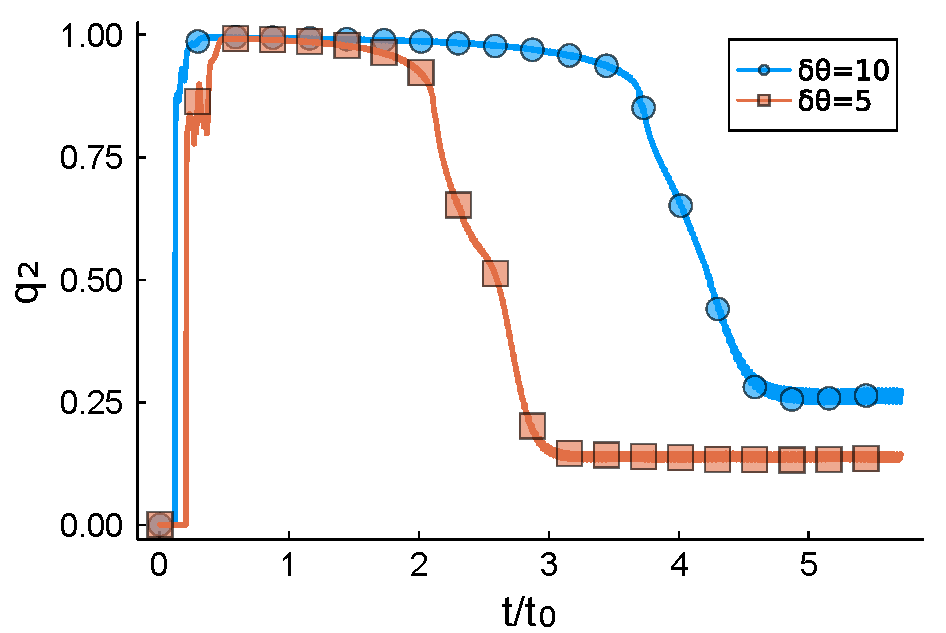
\includegraphics[width=0.4\textwidth]{SupMatFig_2.pdf}
    \caption{LEFT PANEL. Minkowski's structure metric $q_2$ for three different wavelengths $\lambda=64 h_0$, $\lambda=128 h_0$ and 
    $\lambda=256 h_0$ (as in figure 4 of the main text) and for $\Gamma=1.5$ (all other parameters are as in the main text). 
    The time interval during which $q_2 \approx 1$ signals the emergence of rivulets, also for $\lambda = 64 h_0$ which is comparable with the spinodal wavelength $\lambda_s \approx 70 h_0$. RIGHT PANEL. Comparison of the Minkowski's structure metric $q_2$ for $\delta\theta=5^{\circ}$ and $\delta\theta=10^{\circ}$, 
    $\Gamma = 15$ and $\lambda = 256 h_0$.}
    \label{fig:q2_difflambda}
\end{figure}
\noindent In this section we test the robustness of the observation of the rivulet state over a wider parameter space and in particular at changing: 1) the pattern wavelength $\lambda$ and 2) the heterogeneity amplitude $\delta \theta$.
To this aim we have run simulations with $\Gamma=1.5$, $\lambda/h_0 = 64, 128$, and with $\Gamma = 15$, $\lambda = 256 h_0$, $\delta \theta = 5^{\circ}$, respectively.
In Fig.~\ref{fig:q2_difflambda} (left panel) we report the measurements of the Minkowski's structure metric $q_2$, whose increase from zero up to a plateauing value of $q_2 \approx 1$ indicates the emergence of rivulets, for the different $\lambda$'s ($\lambda=256 h_0$, which is the value considered in the main text, is also reported for comparison).
Analogously, in the right panel, we report $q_2$ as a function of time for $\delta \theta = 5^{\circ}$  and $\delta \theta = 10^{\circ}$ (the value used in the main text). 
We see that the $q_2$ metric attains the value $q_2 \approx 1$, signalling the rivulet state, albeit over a time interval shorter than for $\delta \theta = 10^{\circ}$, i.e. the rivulets' lifetime decreases with $\delta \theta$. 
This was somehow expected, since obviously (and also in the static case) the patterning looses effectiveness as the contact angle mismatch is reduced (see, e.g.~\cite{konnurInstabilityMorphologyThin2000}).
%\newpage

\section{Droplet shape}\label{sec:SMdroplet}

\noindent We investigate, here, how the local contact angle of droplets, formed on the more hydrophilic patches after dewetting, depends on the pattern wavelength. 
We recall, in fact, that the patterning is such that the contact angle is not piecewise constant, but varies with continuity.
The droplet shape is determined by minimization of the total interfacial energy
\begin{equation}\label{eq:energy}
E = \gamma_{\text{lg}} A_{\text{lg}} + \int_{A_{\text{sl}}} (\gamma_{\text{sl}} - \gamma_{\text{sg}})d \sigma,
\end{equation}
where $A_{\text{lg}}$ and $A_{\text{sl}}$ are the liquid/gas and solid/liquid interface areas, and $\gamma_{\text{lg}}$, $\gamma_{\text{sl}}$, $\gamma_{\text{sg}}$ are the liquid/gas, solid/liquid and solid/gas interface energies per unit area~\cite{wuHowChemicalPatterns2020}. 
In particular, $\gamma_{\text{lg}} \equiv \gamma$ is the surface tension.
Setting $A_{\text{lg}} \equiv A$ and $A_{\text{sl}} \equiv S$, by Young's equation $\cos \theta = \frac{\gamma_{\text{sg}} - \gamma_{\text{sl}}}{\gamma}$, Eq.~(\ref{eq:energy}) can be rewritten as
\begin{equation}\label{eq:energyoung}
\tilde{E} \equiv \frac{E}{\gamma} = A - \int_S \cos \theta \text{d}x \text{d}y.
\end{equation}
Droplets will form around minima of the contact angle pattern
\begin{equation}\label{eq:contact}
\theta(x,y) = \theta_0 + \delta \theta \sin(q_{\theta} x) \sin (q_{\theta} y) \qquad q_{\theta} = \frac{2\pi}{\lambda},
\end{equation}
namely $(x_n,y_n) = \left((2n+1)\frac{\lambda}{4},(2n+3)\frac{\lambda}{4}\right)$, with $n=0,\pm 1, \pm 2,\dots$.
If we consider large wavelengths ($q_{\theta} h_0 \ll 1$) and heterogeneity ($\delta \theta \ll 1$) such that the contact angle gradients are small, the expression (\ref{eq:contact}) can be expanded as
\begin{equation}\label{eq:contact2}
\theta(x,y) \approx \theta_m + \delta \theta q_{\theta}^2 ((x-x_n)^2 + (y - y_n)^2) + o(|\mathbf{x}-\mathbf{x}_n|^2),
\end{equation}
where $\theta_m = \theta_0 - \delta \theta$.
This local radial symmetry allows to approximate the equilibrium droplet shape as a spherical cap of height $h$ and base radius $a$, whose area is $A = \pi(a^2 + h^2)$; inserting the expression for $A$ and (\ref{eq:contact2}), neglecting higher than second order terms, in (\ref{eq:energyoung}) gives
\begin{equation}\label{eq:energy3}
  \tilde{E}(h,a) = \pi(a^2 + h^2) -
  \int_{\mathcal{C}_a(\mathbf{x}_n)} \cos\left[\theta_m + \delta \theta q_{\theta}^2 ((x-x_n)^2 + (y - y_n)^2)\right]
    \text{d}x\text{d}y,
\end{equation}  
where
$\mathcal{C}_a(\mathbf{x}_n)=\{(x,y) \in [0, L]^2|(x-x_n)^2 + (y-y_n)^2 \leq a^2\}$ is the circle of centre $\mathbf{x}_n$ and radius $a$. 
Due to global volume conservation and assuming the droplets to be monodisperse, the droplet volume is $V_d = h_0L^2/N_d = h_0 \lambda^2/2$, where $N_d$ is the number of droplets, which equals the number of minima of (\ref{eq:contact}) in the domain $[0, L]^2$, i.e. $N_d = 2(L/\lambda)^2$.
Enforcing the volume of the spherical cap to be equal to $V_d$ relates $h$ and $a$ by
\begin{equation}
\frac{\pi h}{6}(3a^2 + h^2) \approx \frac{\pi}{2} a^2 h =  \frac{h_0 \lambda^2}{2}    
\end{equation}
in the ``lubrication approximation'' $h \ll a$, whence
\begin{equation}
  h \approx \left(\frac{h_0}{\pi}\right) \left(\frac{\lambda}{a}\right)^2.
\end{equation}  
Inserting the latter expression in (\ref{eq:energy3}) and performing the integral, the energy (that we indicate now as $E(a)$ to lighten the notation) reads
\begin{equation}\label{eq:energy4}
  E(a) = \pi \left(a^2 + \frac{h_0^2 \lambda^4}{\pi^2 a^4} \right) - \frac{2\pi}{\delta \theta q_{\theta}^2}
  \left[\sin\left(\theta_m +\frac{\delta \theta}{2}q_{\theta}^2a^2\right) - \sin \theta_m \right].
\end{equation}  
We expand, then, the sine in the second term up to second order in $\delta \theta$ (such that the energy is first order) and we finally get
\begin{equation}\label{eq:energyfin}
  E(a) \approx  \pi \left((1-\cos \theta_m) a^2 + \frac{h_0^2 \lambda^4}{\pi^2 a^4} \right)
  + \delta \theta \frac{\pi}{4}\sin \theta_m q_{\theta}^2 a^4 \equiv E_0(a) + \delta \theta E_1(a).
\end{equation}  
The minimum condition $\frac{\partial E}{\partial a} = 0$~\footnote{It can be easily checked that 
$\frac{\partial^2 E}{\partial a^2} > 0$.} yields   
\begin{equation}\label{eq:minim}
2\pi (1-\cos \theta_m)a^6 - 4h_0 \lambda^4 + \delta \theta \pi^2 \sin \theta_m q_{\theta}^2 a^8 =0.
\end{equation}  
The solution of (\ref{eq:minim}) at zero-th order in $\delta \theta$ is
\begin{equation}\label{eq:a0}
  a_0 = \left[\frac{2h_0\lambda^4}{\pi^2(1-\cos \theta_m)}\right]^{1/6}.
\end{equation}
To this order the droplet contact angle $\tan (\theta_d/2) = h/a$ reads
\begin{equation}
\tan \left(\frac{\theta_d}{2}\right) = \frac{h}{a} \approx
\left(\frac{h_0}{\pi}\right)\frac{\lambda^2}{a_0^3} =
\left(\frac{1-\cos \theta_m}{2}\right)^{1/2}\frac{\lambda^2}{(\lambda^{2/3})^3} \approx \frac{\theta_m}{2} \quad \Rightarrow \quad \theta_d \approx \theta_m,
\end{equation}
i.e., it does not depend on $\lambda$. 
We move, then, to the next order. 
We seek a solution to (\ref{eq:minim}) in the form $a = a^{(0)} + \delta \theta a^{(1)} + \dots$, where $a^{(0)} \equiv a_0$.
At the first order in $\delta \theta$ we get
\begin{equation}
a^{(1)} = -q_{\theta}^2 a_0^3\frac{\sin \theta_m}{6(1-\cos \theta_m)},
\end{equation}
such that the correction to the droplet contact angle provides
\begin{equation}
  \tan \left(\frac{\theta_d}{2}\right) \approx \frac{h_0 \lambda^2}{\pi a_0^3}
  \left(1+\delta \theta q_{\theta}^2 a_0^2 \frac{\sin \theta_m}{12(1-\cos \theta_m)}\right)
  \quad \Rightarrow \quad \theta_d \approx
  \theta_m \left(1+\frac{\delta \theta}{\theta_m}\frac{b}{\lambda^{2/3}}\right),
\end{equation}  
where $b = \left(\frac{32 h_0^2 \pi^4}{27 \theta_m^5}\right)^{1/3}$, i.e. the droplet contact angle grows at decreasing pattern wavelength as $\theta_d \sim \lambda^{-2/3}$.

\bibliography{betterRef}

%\begin{thebibliography}{99}

%\bibitem{konnurInstabilityMorphologyThin2000} R. Konnur, K. Kargupta and A. Sharma, {\it Phys. Rev. Lett.} {\bf %84}, 931--934 (2000).
%\bibitem{WuSM2020} Y. Wu, F. Wang, S. Ma, M. Selzer and B. Nestler,
%{\it Soft Matter} {\bf 16}, 6115--6127 (2020).
%\bibitem{footnote} It can be easily checked that $\frac{\partial^2 E}{\partial a^2} > 0$ %for $a>0$.
  
%\end{thebibliography}

\end{document}
